\chapter{Reinforcement Learning and Deep Neural Networks}
\label{ch:reinforcement_learning}

\begin{remark}{Outline}

\end{remark}

\section{Introduction}
\label{sec:rl_introduction}


\section{Markov Decision Processes}
\label{sec:mdps}

In order to develop and apply RL algorithms to optimal decision making problems, we need to formulate the problem in a specific framework: in RL this is done with Markov Decision Processes (MDPs). Throughout this thesis we will characterize MDPs, and the resulting RL concepts, by using the mathematical notation that was used by \citet{sutton2018reinforcement} in their seminal book about RL, although it is worth noting that within the literature, different formulations can be found to express the same kind of concepts \cite{busoniu2010reinforcement}.

We start by introducing the following elements:
\begin{itemize}
	\item A set of possible states $\mathcal{S}$, that can be visited by an agent while it is interacting with the MDP, where $s_t \in \mathcal{S}$ denotes the state being visited at time-step $t$.
	\item A set of possible actions $\mathcal{A}$ that are available to the agent when it is in a certain state, where $a_t \in \mathcal{A}(s_t)$ denotes the action that is performed by the agent in state $s$ at time-step $t$.
\item A transition function $\mathcal{P}:\matchal{S}\times\matchal{A}\times\matchal{S}\Rightarrow [0,1]$ that defines the probability for an agent to visit state $s_{t+1}$, based on its current state and the action which will be performed thereafter. This probability is then defined as $p(s_{t+1}|s_t, a_t)$.
\item A reward function $\mathcal{R}:\matchal{S}\times\matchal{A}\times\matchal{S}\Rightarrow \mathbb{R}$ which returns a reward signal $r_{t+1}$ when an agent performs action $a_t$ in state $s_t$ and transits to $s_{t+1}$.
\item A discount factor denoted as $\gamma \in [0,1]$.

\end{itemize}

Based on these concepts a MDP is then defined by the following tuple $<\mathcal{S}, \matchcal{A}, \matchal{P}, \mathcal{R}, \gamma>$ and is also commonly denoted in the RL literature as the \textbf{environment}. The way the agent interacts with this environment is defined by its \textbf{policy} $\pi$, defined as
\begin{equation}
	\pi(a|s) = \text{Pr}\; \{A_t = a | S_t = s\}, \; \text{for all}\; s \in \mathcal{S}\; \text{and}\; a\ \in \mathcal{A} 
\end{equation}
which maps each state to an action $\pi:\mathcal{S}\Rightarrow\mathcal{A}$.

The elements of a MDP allow us to properly model the dynamics of an agent interacting with its environment, an interaction which can be summarized as follows: at each time-step $t$ the environment provides the agent with a certain state $s_t$, the agent then performs action $a_t$ which results into the reward signal $r_{t+1}$. After performing such action the agent will enter into a new state $s_{t+1}$. This continuous interaction with the environment is also known as the Reinforcement Learning loop, and can technically be infinite. This is however never the case in practice, since an agent will eventually visit a state which only transits to itself (denoted as terminal), which will therefore stop the agent-environment interaction. We visually represent the Reinforcement Learning loop in Fig. \ref{fig:rl_loop}.

\begin{figure}[ht!]
\centering
  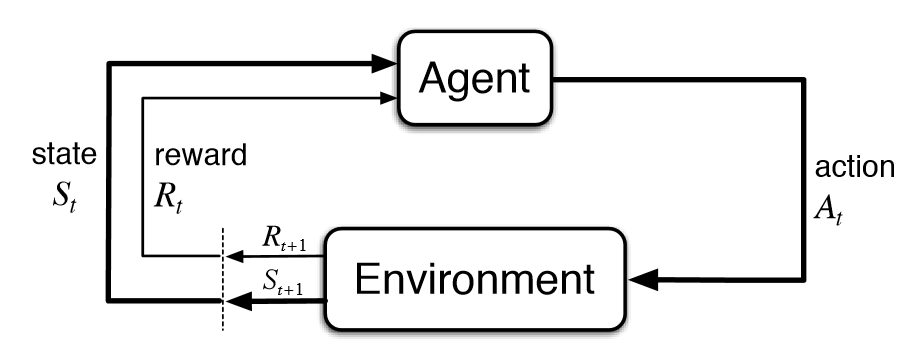
\includegraphics[width=10cm]{./Images/Chapter06/rl_loop.png}
  \caption{A visual representation of how an agent interacts with an environment as modeled by a Markov decision process. Figure taken from page 48 of the \citet{sutton2018reinforcement} textbook.}
  \label{fig:rl_loop}
\end{figure}

Each interaction of the agent with the environment is defined as an \textbf{episode}, which consists of one, or several trajectories $\tau$ that come in the form of the following sequence:
\begin{align}
	\langle(s_t,a_t,r_t,s_{t+1})\rangle,t=0,\dotsb,T-1
\end{align}
where $T$ is a random variable representing the length of the episode.

A key property of the environment is that it fulfills the Markov property which is defined as follows:
\begin{definition}
	A discrete stochastic process has the Markov property if the conditional distribution of the next state of the process only depends from the current state of the process.
\end{definition}
This implies that the only information that is necessary for predicting to which state an agent will step next are $s_t$ and $a_t$, which can be expressed formally as:
\begin{align}
	p(s_{t+1}|s_t, a_t, s_{t-1}, a_{t-1}, \dotsb) = p(s_{t+1} | s_t, a_t).
\end{align}
Interestingly, a similar conclusion also holds for the reward that the agent will get, meaning that the reward that is obtained by an agent is only determined by its previous action, and not by the history of all previously taken actions, as defined by:
\begin{align}
	(r_t| s_t, a_t, \dotsb, s_1, a_1) = p(r_t|s_t,a_t).
\end{align}

\section{Goals and Returns}
So far we have defined all the elements that model the interaction of an agent with an environment, whilst introducing some key properties that are key for the development of RL algorithms. While it is true that we have defined how the agent-environment interaction works, we yet do not know what the purpose of this interaction is. In RL the goal of an agent is defined with respect to the reward signal $r_t$ that is returned by the reward function $\mathcal{R}$. Informally, the goal of an agent is that of maximizing the total amount of reward it receives while interacting with the environment. In the simplest case we can define this as:
\begin{align}
	G_t = r_t, r_{t+1}, r_{t+2}, \dotsb, r_{T}.
\label{eq:goal}
\end{align}
While simple and intuitive this formulation has one major drawback: it treats each reward signal equally since it does not distinguish rewards that are obtained in the near future, i.e. $r_t$, from the ones that will be obtained in the distant future, i.e. $r_{T-1}$. To deal with such issue we need an additional concept known as \textbf{discounting}, which is governed by the discount rate parameter $\gamma$ also known as the discount factor. $\gamma$ allows us to weight the different reward signals an agent receives based on how close or distant in the future these rewards are received by the agent. By introducing $\gamma$ in Eq. \ref{eq:goal} we can define the expected discounted return as:
\begin{align}
G_t = r_t+\gamma r_{t+1}, \gamma^{2} r_{t+2} + ... \\
= \sum_{k-0}^{\infty}\gamma^{k} r_{t+k+1}.
\end{align}

\section{Value Functions}


\section{Learning Value Functions}
\subsection{Monte Carlo Methods}
\subsection{Temporal Difference Learning}

\section{Function Approximators}
\subsection{Linear Functions}

\subsection{Deep Neural Networks}

\section{}
